\begin{figure}[h]
    \centering
    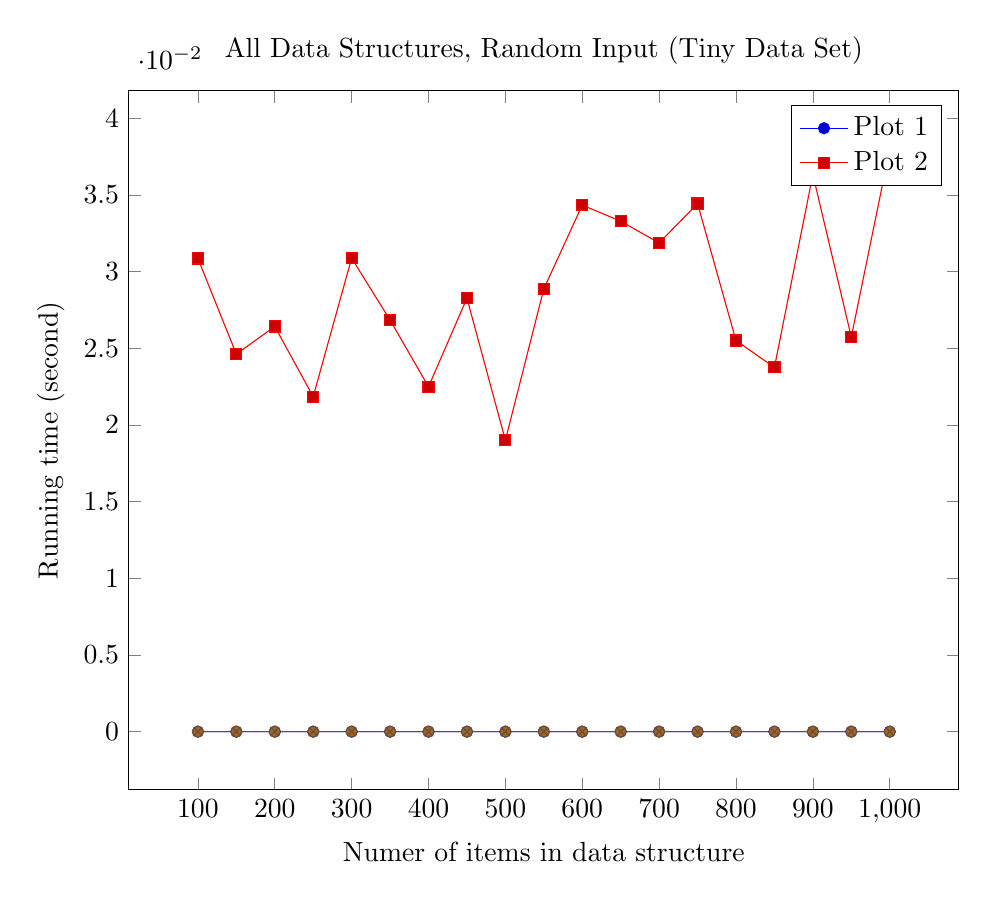
\begin{tikzpicture}
        \begin{axis}[
            xlabel={Numer of items in data structure},
            ylabel={Running time (second)},
            title={All Data Structures, Random Input (Tiny Data Set)},
            width=\textwidth
        ]
		\addplot coordinates {
			(100, 5.42115606152957e-06)
			(150, 5.541626196230165e-06)
			(200, 5.541626196230859e-06)
			(250, 5.391038527854941e-06)
			(300, 5.631978797256132e-06)
			(350, 6.384917139135721e-06)
			(400, 6.294564538109754e-06)
			(450, 5.96327166768329e-06)
			(500, 6.4752697401609934e-06)
			(550, 5.903036600332645e-06)
			(600, 5.722331398281405e-06)
			(650, 5.662096330931455e-06)
			(700, 5.96327166768329e-06)
			(750, 5.963271667682596e-06)
			(800, 5.872919066657323e-06)
			(850, 6.2644470044351254e-06)
			(900, 5.933154134007967e-06)
			(950, 6.1138593360592075e-06)
			(1000, 5.872919066658016e-06)
		};
		\addplot coordinates {
			(100, 0.030848817510334213)
			(150, 0.02461412662917013)
			(200, 0.02641572737608584)
			(250, 0.021842349769977433)
			(300, 0.030870682839781692)
			(350, 0.02683553567798356)
			(400, 0.0224856904068119)
			(450, 0.028263257361854244)
			(500, 0.018999495531312506)
			(550, 0.028866330856166654)
			(600, 0.034329079231701344)
			(650, 0.03328080835460412)
			(700, 0.03186058593661869)
			(750, 0.03442801532982429)
			(800, 0.025500033882225638)
			(850, 0.023748157183408124)
			(900, 0.03632400442727857)
			(950, 0.02572784290694443)
			(1000, 0.037971855164779814)
		};
		\addplot coordinates {
			(100, 6.776445076184245e-06)
			(150, 7.4390308157035175e-06)
			(200, 5.903036600329869e-06)
			(250, 5.391038530433434e-06)
			(300, 6.2945645368017725e-06)
			(350, 6.896915209608778e-06)
			(400, 5.963271667042136e-06)
			(450, 6.3246820730000765e-06)
			(500, 6.62585741224575e-06)
			(550, 7.198090548854452e-06)
			(600, 5.692213863994766e-06)
			(650, 6.776445076184245e-06)
			(700, 7.137855476457844e-06)
			(750, 6.505387278821217e-06)
			(800, 7.860676288373724e-06)
			(850, 6.716210009471979e-06)
			(900, 5.6018612610841956e-06)
			(950, 6.475269742622913e-06)
			(1000, 6.776445076184245e-06)
		};
        \legend{Plot 1, Plot 2}
        \end{axis}
    \end{tikzpicture}
    \caption{Average of 10 operations, benchmarked every 50, starting at 100. Median of 11 runs.}
\end{figure}